\documentclass[
	ngerman,
	fontsize=10pt,
	parskip=half,
	titlepage=true,
	DIV=12
]{scrartcl}

\usepackage[utf8x]{inputenc}
\usepackage{babel}
\usepackage[T1]	{fontenc}
\usepackage{lmodern}
\usepackage{microtype}
\usepackage{color}
\usepackage{csquotes}
\usepackage{amsmath}
\usepackage{hyperref}

\usepackage{minted}
	\usemintedstyle{xcode}

\usepackage{wrapfig}
\usepackage{graphicx}
\usepackage[bf]{caption} 
	\captionsetup{format=plain}

\usepackage{minted}
	\usemintedstyle{xcode}
	
\begin{document}

\part*{C-Kurs, Blatt 06, WiSe 2020}

\section{Integrator (2P)}
\begin{wrapfigure}{r}{.3\linewidth}
	\vspace{-50pt}
	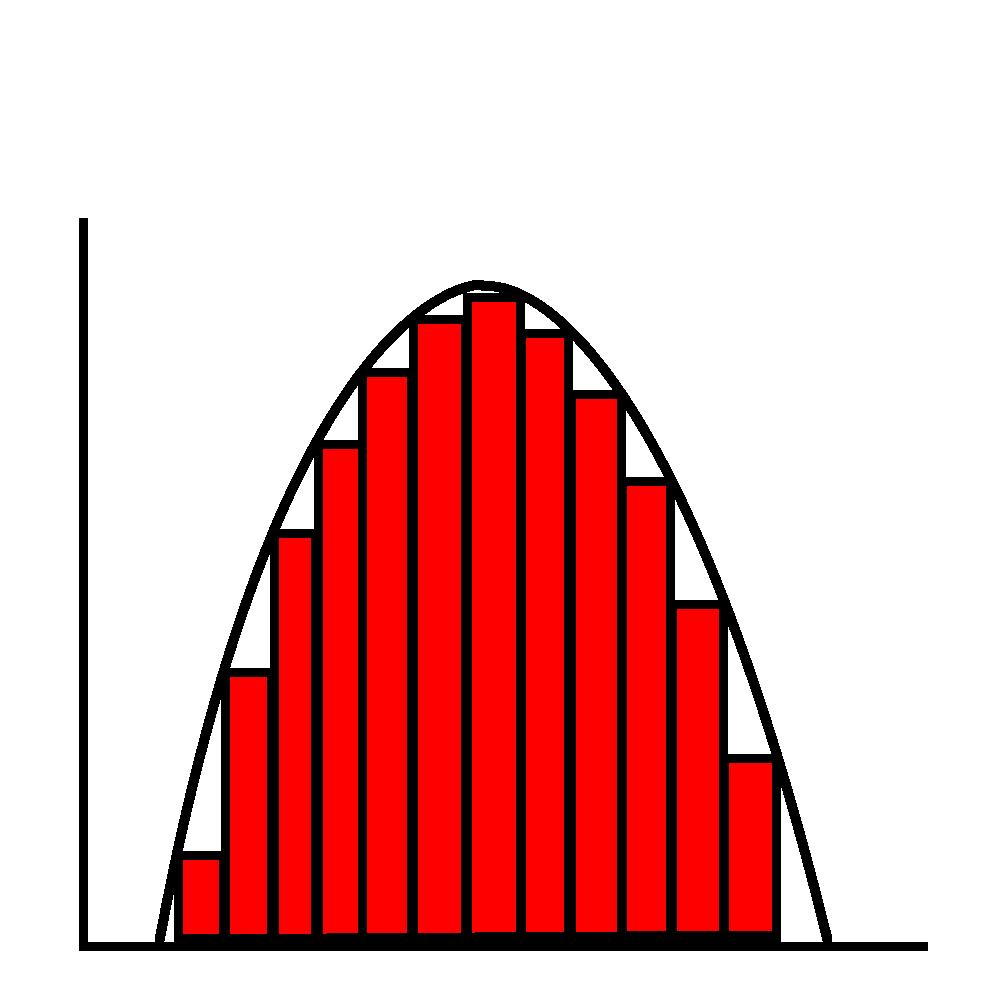
\includegraphics[width=\linewidth]{./integral}
	\caption{Näherung des Integrals durch Rechtecke.\newline
		Bildquelle: \url{https://www.wyzant.com/resources/lessons/math/calculus/integration}}
	\vspace{-50pt}
\end{wrapfigure}
Schreiben Sie eine Funktion, die die Fläche unter einem Graphen näherungsweise berechnet. Der Integrand (also die Funktion zum Graphen) soll als Parameter übergeben werden können. Ihre Funktion soll also folgende Signatur besitzen:
\begin{minted}{c}
double integrate(
   double (*func)(double), 
   double from, 
   double to, 
   int    N
);
\end{minted}

Nutzen Sie dazu die Rechteck-Näherung:
\begin{itemize}
\item Zerlegen Sie den Integrationsbereich in $N$ Intervalle gleicher Breite
\item Finden Sie zu jedem Intervall den Funktionswert des Integranden. Dies sind die Höhen der Rechtecke
\item Bestimmen Sie die Flächen der $N$ Rechtecke und summieren Sie diese auf -- dies ist die Näherung des Integrals.
\end{itemize}

Zum Testen können Sie folgenden Aufruf versuchen:
\mint{c}{printf("%lf\n", integrate(exp, 0, 1, 10000));}
Die Ausgabe sollte in der Nähe von \texttt{1.718} liegen.

\emph{Lernziel: Function Pointers, Schleifen}


\section{Kommandozeilenparameter (1P)}
Schreiben Sie ein Programm, dass das Produkt der Kommandozeilenparamter berechnet. Man soll das fertige Programm also so aufrufen können:
%
\begin{center}
\texttt{./multiply 3.4 7.3 9.2 4}
\end{center}
%
und damit folgende Ausgabe bewirken:
%
\begin{center}
\texttt{913.376}
\end{center}

Schreiben Sie das Programm so, dass es für eine beliebige Zahl von Kommandozeilenparametern funktioniert. Bedenken Sie auch, was passiert, wenn der User \emph{keine} Parameter eingibt (Sie könnten dann z.\;B. eine Fehlermeldung ausgeben).

Tipp: Die Funktion \texttt{atof} wandelt Strings in \mintinline{c}{double}s um. Sehen Sie sich in der CPP-Referenz die Details zu diesem Befehl an.

\emph{Lernziel: Kommandozeilenparameter}


\section{\texttt{qsort} (2P)}
Befüllen Sie ein Array mit Zufallszahlen. Benutzen Sie danach den Befehl \texttt{qsort}, um diese aufsteigend nach ihrer Quersumme zu sortieren. Sie können dazu Ihren Quersummen-Code von Blatt 3 benutzen.

Beispiel: Die Liste
\begin{center}
\texttt{10 15 20 25 30}
\end{center}
%
sollte so sortiert werden:
%
\begin{center}
\texttt{10 20 30 15 25}
\end{center}

\emph{Lernziel: Funktionszeiger}


\section{Text-Trimmen (1P)}
Schreiben Sie ein Programm, das aus einem Text alle mehrfach vorkommenden
Leerzeichen entfernt und den Text auf dem Bildschirm ausgibt.

Beispiel: Die Eingabe:
\begin{verbatim}
   Ein   Text mit     vielen     Leerzeichen
\end{verbatim}
%
soll zu der Ausgabe
%
\begin{verbatim}
Ein Text mit vielen Leerzeichen
\end{verbatim}
führen.

\emph{Lernziel: Arbeiten mit Arrays}


\section{Optional: Structs und Macros (2P)}
\begin{wrapfigure}{r}{.25\linewidth}
	\vspace{-40pt}
	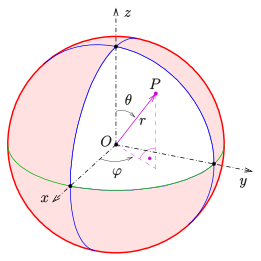
\includegraphics[width=\linewidth]{./Kugelkoordinaten}
	\caption{Von Wikipedia-User Ag2gaeh, CC BY-SA 4.0,\\
		\url{https://commons.wikimedia.org/w/index.php?curid=41627945}}
	\label{fig:Spericals}
\end{wrapfigure}
Benutzen Sie das \texttt{struct vector3d\_t} aus Blatt 5, Aufgabe 1, und lösen Sie folgende Aufgaben mit Makros:
\begin{itemize}
\item Schreiben Sie ein Makro \texttt{ASSIGN(vec, x, y, z)}, mit dem Sie in einer Anweisung alle drei
	Komponenten festlegen können.
\item Berechnen Sie die kartesische Form eines Vektors aus seinen Kugelkoordinaten.\\
	Kugelkoordinaten haben die Komponenten $r$, $\varphi$, $\theta$. Dabei ist $r$ die Länge des Vektors,
	$\varphi$ der Winkel, den seine Projektion auf die $x,y$-Ebene mit der $x$-Achse einschließt und 
	$\theta$ der Winkel, den der Vektor mit der $z$-Achse bildet. Vgl. hierzu Abb.\,\ref{fig:Spericals}
\end{itemize}

\emph{Lernziel: Makros}
\end{document}